\let\negmedspace\undefined
\let\negthickspace\undefined
\documentclass[journal]{IEEEtran}
\usepackage[a5paper, margin=10mm, onecolumn]{geometry}
%\usepackage{lmodern} % Ensure lmodern is loaded for pdflatex
\usepackage{tfrupee} % Include tfrupee package

\setlength{\headheight}{1cm} % Set the height of the header box
\setlength{\headsep}{0mm}     % Set the distance between the header box and the top of the text

\usepackage{gvv-book}
\usepackage{gvv}
\usepackage{cite}
\usepackage{amsmath,amssymb,amsfonts,amsthm}
\usepackage{algorithmic}
\usepackage{graphicx}
\usepackage{textcomp}
\usepackage{xcolor}
\usepackage{txfonts}
\usepackage{listings}
\usepackage{enumitem}
\usepackage{mathtools}
\usepackage{gensymb}
\usepackage{comment}
\usepackage[breaklinks=true]{hyperref}
\usepackage{tkz-euclide} 
\usepackage{listings}
% \usepackage{gvv}                                        
\def\inputGnumericTable{}                                 
\usepackage[latin1]{inputenc}                                
\usepackage{color}                                            
\usepackage{array}                                            
\usepackage{longtable}                                       
\usepackage{calc}                                             
\usepackage{multirow}                                         
\usepackage{hhline}                                           
\usepackage{ifthen}                                           
\usepackage{lscape}
\begin{document}

\bibliographystyle{IEEEtran}
\vspace{3cm}

\title{4.11.37}
\author{EE25BTECH11060 - V.Namaswi}
% \maketitle
% \newpage
% \bigskip
{\let\newpage\relax\maketitle}
\renewcommand{\thefigure}{\theenumi}
\renewcommand{\thetable}{\theenumi}
\setlength{\intextsep}{10pt} % Space between text and floats
\textbf{Question}\\Show that the lines $\frac{x-1}{3}=\frac{y-1}{-1}=\frac{z+1}{0}$  and $\frac{x+4}{2}=\frac{y}{0}=\frac{z+1}{3}$ intersect.Find their point of intersection.\\
\textbf{Solution}\\
Let,
\begin{align}
\frac{x-1}{3}=\frac{y-1}{-1}=\frac{z+1}{0}=\lambda\\
\frac{x+4}{2}=\frac{y}{0}=\frac{z+1}{3}=\mu
\end{align}
 To check point of intersection,
 \begin{align}
     \begin{pmatrix}
         1 \\ 1 \\ -1 
     \end{pmatrix}+\lambda \begin{pmatrix}
         3 \\ -1 \\ 0
     \end{pmatrix}=\begin{pmatrix}
         -4 \\ 0 \\ -1 
     \end{pmatrix}+ \mu \begin{pmatrix}
         2 \\ 0 \\ 3
     \end{pmatrix}\\
     \implies \begin{pmatrix}
         3 & -2 \\ -1 & 0 \\ 0 & -3 
     \end{pmatrix}\begin{pmatrix}
         \lambda \\ \mu
     \end{pmatrix}=\begin{pmatrix}
         -5 \\ -1 \\ 0
     \end{pmatrix}\\
 \end{align}
 Using gaussian elimination\\
 Argumented matrix\\
 \begin{align}
     \begin{bmatrix}
         3 & -2 &  | & -5 \\
         -1 & 0  & | & -1\\
         0 & -3 & | & 0 
     \end{bmatrix}
 \end{align}
 Apply the row operation \( R_2 \to 3R_2 + R_1 \):
\begin{align}
\begin{bmatrix}
3 & -2 & | & -5\\
0 & -2 & | & -8\\
0 & -3 & | & 0
\end{bmatrix}
\end{align}

Divide the second row by \(-2\):
\begin{align}
\begin{bmatrix}
3 & -2 & | & -5\\
0 & 1  & | & 4\\
0 & -3 & | & 0
\end{bmatrix}
\end{align}

Now eliminate using \(R_2\):  
\[
R_1 \to R_1 + 2R_2, 
\quad R_3 \to R_3 + 3R_2
\]

\begin{align}
\begin{bmatrix}
3 & 0 & | & 3\\
0 & 1 & | & 4\\
0 & 0 & | & 12
\end{bmatrix}
\end{align}
 The last row gives \(0 = 12\), which is a contradiction.  
Hence, the system is inconsistent and has \textbf{no solution}.  
Therefore, the two lines are skew and do not intersect.
\begin{align}
\centering
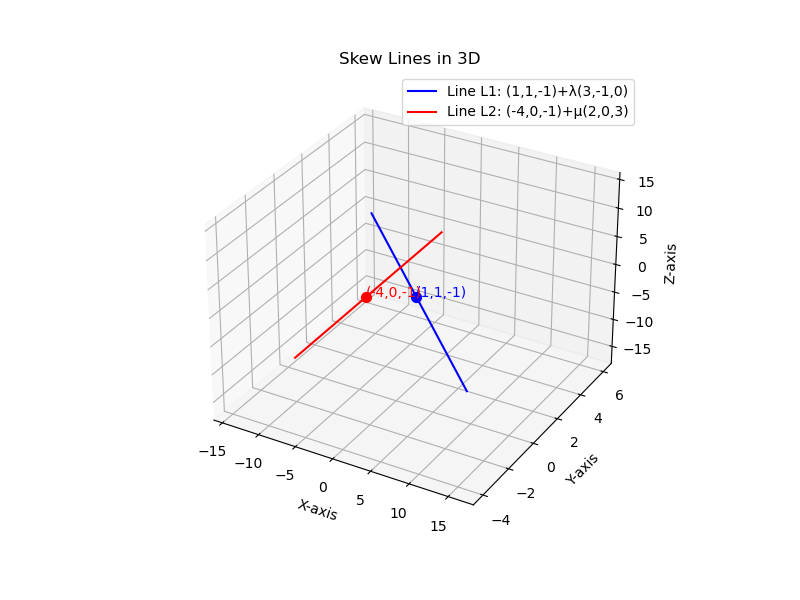
\includegraphics[width=\columnwidth, height=0.8\textheight, keepaspectratio]{figs/Figure_8.png}       
\end{align}
\end{document}